\documentclass[12pt,oneside]{book}
\usepackage[T1]{fontenc}
\usepackage{geometry}
\usepackage{epsfig}
\geometry{verbose,a4paper,tmargin=25mm,bmargin=25mm,lmargin=32mm,rmargin=32mm}
\usepackage{graphicx}
\usepackage{setspace}
\usepackage{amsmath}
\usepackage{enumerate}
\usepackage{amssymb}
\usepackage{caption}
\usepackage{array}
\usepackage{tabu}
\usepackage[utf8]{inputenc}
\setcounter{secnumdepth}{5}
\setcounter{tocdepth}{5}
\onehalfspacing
\usepackage{txfonts}
%\usefont{T1}{tnr}{m}{sl}
\makeatletter
\makeatother
\renewcommand{\contentsname}{TABLE OF CONTENTS}
\renewcommand\listtablename{LIST OF TABLES}
\renewcommand\listfigurename{LIST OF FIGURES}
\renewcommand\bibname{REFERENCES}
\usepackage[authoryear,round]{natbib}
\renewcommand{\chaptername}{CHAPTER}
%\renewcommand{\section}{\MakeUppercase}
%\usepackage[authoryear,round]{natbib}
%\usepackage[options]{natbib}
\newtheorem{definition}{Definition}
 
\title{}
\author{}
\thispagestyle{empty}
\begin{document}
\begin{titlepage}
\begin{center}
{\LARGE \bf A Hybrid Matchmaking Engine Using Advanced Recommender System } \\
\end{center}
\begin{center}
%\vspace{0.2in}
%{\large Dissertation} \\
\vspace{0.6in}
{\large \it A project report submitted in partial fulfillment of the requirements for B.Tech. Project} \\
\vspace{0.6in}
{\large \bf B.Tech.} \\
\vspace{0.5in}
{\large \it by\\}
\vspace{0.3in}
{\large \bf  K. Shashank (2014IPG-047)}\\
%{\normalsize (2014IPG-47)}\\
{\large \bf  P. Akhilesh Naik (2014IPG-111)}\\
%{\normalsize (2014IPG-111)}\\
{\large \bf Jk. Snehith (2014IPG-121)}\\
%{\normalsize }\\
\end {center}
\vspace{0.8in}
\begin{figure}[h]
\centerline{
\includegraphics[width=1.2in]{dwd.jpg}}
\end{figure}
%\vspace{0.1in}
\begin{center}
{\Large \bf ABV INDIAN INSTITUTE OF INFORMATION TECHNOLOGY AND MANAGEMENT\\
GWALIOR-474 010\\}
\vspace{0.2in}
{\Large \bf 2017\\}
\end{center}
\end{titlepage}
\setcounter{page}{1}
\pagenumbering{roman}
\newpage
\begin{center}
{\large \bf CANDIDATES DECLARATION}
\end{center}
We hereby certify that the work, which is being presented in the report, entitled {\bf A Hybrid Matchmaking Engine Using Advanced Recommender System}, 
in partial fulfillment of the requirement for the award of the
Degree of {\bf Bachelor of Technology} and submitted to the institution is an authentic record of our own work carried out
during the period \emph{May 2017} to \emph{September 2017} under the supervision of {\bf Dr. Pramod Kumar singh}. We also cited the reference about the text(s)/figure(s)/table(s) from where they have been taken.\\
\vspace{0.6in} \\
Date: \hspace{3.4in} Signatures of the Candidates \\
%\begin{flushright}
%Signatures of the Candidates
%\end{flushright}
\vspace{0.2in} \\
This is to certify that the above statement made by the candidates is correct to the best of my knowledge. \\
\vspace{0.5in} \\
Date: \hspace{2.65in} Signature of the Research Supervisor \\
%\begin{flushright}
%Signatures of the Research Supervisors
%\end{flushright}
\newpage
\addcontentsline{toc}{chapter}{ABSTRACT}
\begin{center}
{\large \bf ABSTRACT}
\end{center}
Use of online matrimony for matchmaking is the new norm in India on contemporary to the already existing dating sites with a different notion all together. One fundamental component to realize the perfect match is through ranking of matches. Using content-based approaches we designed two distinct scoring algorithms. This algorithms solve the cold-start problems by being able to provide recommendations immediately based on new user's profiles and preferences. The later part is collaborative filtering which uses the interactions of the similar active users, including the people they like/dislike and are liked/disliked by, to result in reciprocal recommendations. The objective of the following study is to enable users to get their match in a more apt and efficient way for both user as well as the recommender system. So, we also make use of collaborative filtering as to achieve the following above statement. \\

{\it Keywords: Recommender System, Collaborative Filtering, Content Based, AHP}
\newpage
\begin{center}
{\large \bf ACKNOWLEDGEMENTS}
\end{center}
We are highly indebted to {\bf Dr. Pramod Kumar Singh}, and are obliged for giving us the autonomy of functioning and experimenting with ideas. We would like to take this opportunity to express our profound gratitude to them not only for their academic guidance but also for their personal interest in our project and constant support coupled with
confidence boosting and motivating sessions which proved very fruitful and were instrumental in infusing self-assurance
and trust within us. The nurturing and blossoming of the present work is mainly due to their valuable guidance,
suggestions, astute judgment, constructive criticism and an eye for perfection. Our mentor always answered myriad of our
doubts with smiling graciousness and prodigious patience, never letting us feel that we are novices by always lending an
ear to our views, appreciating and improving them and by giving us a free hand in our project. It's only
because of their overwhelming interest and helpful attitude, the present work has attained the stage it has. \\
Finally, we are grateful to our Institution and colleagues whose constant encouragement served to renew our spirit,
refocus our attention and energy and helped us in carrying out this work.\\ \\ \\ \\
%\vspace{0.7in}
( K. Shashank) \hspace{1in} (P. Akhilesh Naik ) \hspace{1in} (Jk. Snehith)
\newpage
 \tableofcontents
\addcontentsline{toc}{chapter}{LIST OF TABLES}
\listoftables
\addcontentsline{toc}{chapter}{LIST OF FIGURES}
\listoffigures
\newpage
\begin{center}
{\large\bf ABBREVIATIONS}
\end{center}
\begin{table}[h!]
\begin{tabular}{p{2cm}p{8cm}}
RS & Recommender System \\
MS & Match-making system \\
AHP & Analytic Hierarchy Process\\
\end{tabular}
\end{table}
\newpage \setcounter{page}{1}
\pagenumbering{arabic}
\chapter{INTRODUCTION AND LITERATURE SURVEY}
This chapter includes the details of recommender systems, concepts of collaborative filtering, purpose of recommender systems in matrimonial sites, how matrimonial sites are different from other domain having various match-making systems, platform used to implement the project and literature review related to work done in this field.
\section{INTRODUCTION}
With the rise in amount of data the choice of selective and required information has always been one of the key problems in today's era.

In such situations recommender systems have paved the way so as to remove the individual burden to make evaluative decision's and reduced overload of information. Almost always the traditional recommender system was used to provide items, information and services in the field of e-commerce.

In many past years Recommendation system that were built utilizing non-personalized, demographic content-based, collaborative filtering and knowledge based RC.\\Further the recommender system have evolved in areas such as social match-making system where a user is meant to meet other user in order to satisfy a particular need. Many match-making systems that exist today include dating services, resume/job bulletin board, consumer to consumer market places. 
\subsection{RECOMMENDER SYSTEMS FOR MATRIMONIAL SITES}
 The role of recommender systems have always played a important part of online dating site as social matchmaking RS which dated back to 1965. During the year 1965 a team of Harvard undergrads created Operation Match, the world's first computer dating service. For 3 Dollar, users could answer questionnaires and receive a list of potential matches, a process that is still used by many dating sites. Online dating sites is a system that enables a user to find and introduce themselves to opposite gender user usually with the goal of developing personal, romantic relationship with a wide variety of un-modulated match-making services. Online dating is the new norm for introductions, replacing the role of traditional personals and in many cases, merging with the functions of social media.
 
 Matrimonial websites are a variation of the standard dating websites popular in India and among Indians settled overseas as an alternative to the traditional marriage broker system that prevailed before online matrimonial sites emerged. Few to name are Bharatmatrimonial.com, shaddi.com and few other Pioneers in the field of social match-making. Despite the popularity of such systems,   relatively little research is done on match-making RS that are used in matrimonial sites
\section{LITERATURE REVIEW}
 The field of recommender systems has garnered a lot of attention in both the industry and academia, with a considerable volume of litereature\cite{4}. It is a prevalent way of solving the information rich problems. They have been popularized by widely popular commercial services such as Netflix\cite{5} or Amazon\cite{6}. Other popular services exploiting the benifits of RS are match.com \cite{7}, Ringo\cite{8}, Bellcore \cite{8}, Pandora, Tripadvisor, PHelp \cite{7}, i-Help \cite{7}, Flipkart, Twitter, Facebook etc. Deshpande $et$ $al$. \cite{9} performed an analysis of various term-based top-n recommendation algorithms on several popular datasets including movies, credit card transactions, and others using different metrics.
\subsection{MATRIMONY MATCHING RECOMMENDER SYSTEM}
Deployment of RS in matrimony is an upcoming area of research. Even though matrimony is considered as a potential application for RS there is a surprising lack of literature published on this problem. Considerable amount of work is done in matchmaking in dating services. A combination of content-based RS and reciprocal algorithm has been implemented in Recon \cite{7} system. User profiles and interactions with other users are used by Recon system as their parameters. This system tried to extract user's onsite preferences which are inferred from his/her communication with users of opposite gender and all the similar profiles are matched with them. Two recommendation engines based on collaborative filtering approaches for an online dating service were developed by Brozosky and Petricek\cite{10} implemented two RS for online dating based on collaborative filtering and tested their algorithm on a real dating service data. The results from their analysis have shown that collaborative filtering based recommender systems outperform popularity based recommender systems. L. Li and T. Li have implemented MEET \cite{11} system for online dating using bipartite graph. A hybrid content-collaborative approach \cite{12} for online dating was put forward by J. Akehurst $et$ $al$.

K. Joshi and S. Kumar \cite{1} were able to use analytical hierarchy process in matrimony to calculate weights for different attributes. A framework \cite{2} for implementation of collaborative filtering in matrimony was provided by Sampath.M.K $et$ $al$. S. Khavate and M. A. Potey \cite{3} came up with partial fuzzy  based scoring system for Indian matrimony.\\
\newpage
\chapter{DESIGN DETAILS AND IMPLEMENTATION}
In this chapter we would like to give an overview of matrimonial site, to analyze and understand the concept of the proposed recommender system and the implementation of algorithm using user rank method and the use of collaborative filtering is explained in the latter part of this chapter.
\section{DESIGN DETAILS}
\subsection{OVERVIEW OF MATRIMONIAL SITE}
Unlike the online dating sites where the users preferences are almost accounted for and a small profile has to be filled to choose your match.The matrimonial site is different because of the intent, purpose  and the requirement that the user wants. Here, users range from self to serious parents and grandparents, search each and and every recommendation with at-most care in hope to find the perfect match for the bride or groom in every recommendations provided to them give.

First, the user of matrimonial sites have to create a profile for himself or the person for whom he/she would want to find a match. This is done by registering into it and giving detail on one's own free will. They must also provide preference details about the partner. User profile will be generated once the user submits the registration form. The user now becomes active user and his preferences about their partner are then taken and matches are identified using collaborative filtering. Now, the user interests are identified by using personalized algorithms and profiles when matched user interests are identified. When the profiles that satisfy both users preferences and interest are now considered for recommendation from this we obtain top n-profiles based on weightage of profiles to each active user. One of the main problem of having only collaborative filtering or reciprocal recommender system is it does not specify the degree of acceptance of one match over other and is  inefficient in terms of giving recommendation to all the active user.

User's profile is a union of both female and male user's in a matrimonial sites now these profiles are further divided into account information, contact information, personal profile and preferred partner's profile. Account information comprises of login name, password, user's name, date of birth and security question and answer. Contact information normally consist of address, city, state, country, mobile number and email-id of the user. Personal profile consists of  attributes like age, height, religion, caste, education, occupation, income, complexion, body type, diet, smoke and drink. The preferred partner profile consist of user's excepted range of age, range of height, range of income, religion, caste, education, occupation, complexion, body-type, diet, smoke and drink. Some times user may not put any preferences to a particular attribute and this means the whole range is said to be accepted such as diet is not preferred to be a specific type then the user's partner can be from an origin having any kind of diet.The other attributes are smoke and drink which are preferred attributes for both female and male. 
\subsection{DOMAIN OVERVIEW OF PROPOSED RECOMMENDER SYSTEM}
\begin{figure}[h]
    \centering
    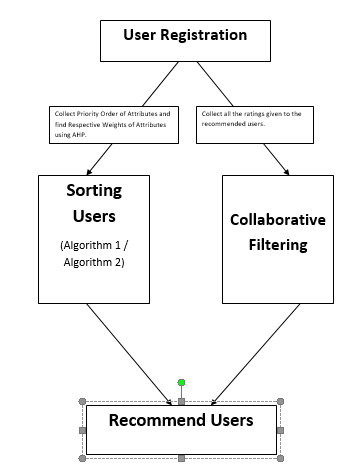
\includegraphics[width=0.75\textwidth]{flow}
    \caption{Proposed System}
    \label{fig:flow}
\end{figure}
1) Creating $user$ $profile$ - New user have to login to the website and give details such as their personal information, contact information and Partner preferences to become an active user.\\\\
2) The attributes are mainly of 12 types which constitutes as  partner's preference list, these 12 attributes are further generalized into 2 groups containing 6 attributes each of HIGH importance and the other 6 attributes of LOW importance.\\\\
3) Then a preference attribute vector is formed to shortlist the matches in N-recommendations.\\\\
4) Browsing other active users for interesting matches.\\\\
5) The users interests on match which is recommended is calculated by the degree of similarity between opposite gender HIGH importance attributes i.e. six attributes which come into the category of HIGH this other LOW category attributes are calculated using Weights of each attribute that the user has given importance to and which in-turn helps in bringing more related recommendations.\\\\
6) The weights for attributes are given using the AHP.\\\\
7) Now Using $collaborative filtering$ - the similarity must be found between the active users and new active users so as to make it efficient by suggesting the same N-recommendation based on degree of similarity in preferences that were provide by both users to find their respective matches.
\section{IMPLEMENTATION}
Content-based and collaborative based filtering are the most common approaches used in recommendation engines. Content-based methods develop user preferences profile based on his/her initial preferences given during signup (e.g. Vegetarian matches in matrimony example) and/or the attributes of the profiles rated positively and/or negatively by the users, the model is based on this data and this model is used to show new profiles that have similar attributes. The techniques based on content-based techniques usually do not take into account the data from other users, they only take the data of the current user into consideration. However well these approaches may address the cold-start problem, the other kind of approaches (collaborative filtering) are more versatile and efficient. These approaches exploit data from other users who gave similar ratings on the same items and recommend items that have been rated positively by other users and not yet by the target user. Both approaches share their own set pros and cons. In our field of online matrimony, the items to be recommended are human beings, who have their own set of preferences, profile and activity in the site. This poses different challenges in giving recommendations as it is considered important to recommend useful recommendations to newly joined users, so that they don't feel bad at the very beginning, hence it becomes critical to solve the cold-start problem. So we decided to come up with two types of algorithms serving different purposes with a common goal to increase user satisfaction by recommending good matches.
The two scoring algorithms discussed in the subsequent section falls in the category of content-based filtering. They only use the preferences of the user while giving recommendations to that user. It is followed by an algorithm based on collaborative filtering which uses the ratings given by other users.
\begin{figure}[h]
    \centering
    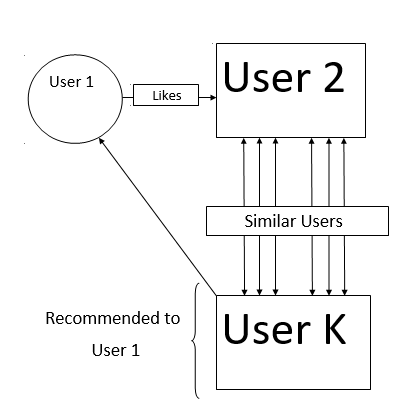
\includegraphics[width=0.5\textwidth]{cb}
    \caption{Content-based approach for matrimony}
    \label{fig:cb}
\end{figure}
\begin{figure}[h!]
    \centering
    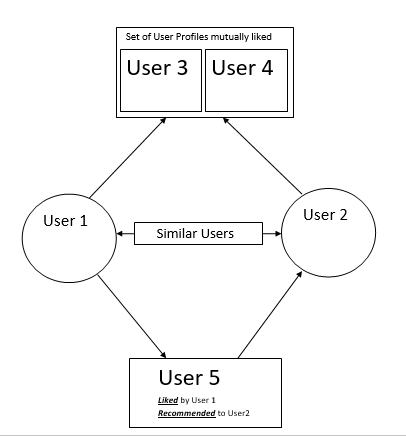
\includegraphics[width=0.5\textwidth]{cf}
    \caption{Collaborative filtering based approach}
    \label{fig:cf}
\end{figure}

\subsection{ANALYTIC HIERARCHY PROCESS (AHP)}
The Analytic Hierarchy Process (AHP) is an effective tool for dealing with complex Multi-Criteria decision making framework and assists the decision maker to derive ratio scales from paired comparisons or by setting priorities and synthesize the results. The  AHP can intake both subjective measurement such as satisfaction feelings, preference and objective/Actual measurements such as price, weight etc of a decision. In addition, the AHP includes a useful technique for checking the conformity or regularity of the decision maker's evaluations, thus reducing the prejudice in the decision making process.
\subsubsection{HOW THE AHP WORKS}
The AHP  takes a set of evaluation attribute into account.The AHP generates a weight for each evaluation attribute according to the decision maker's pairwise comparisons of the attribute. The higher the weight, the more important the corresponding attribute.
\subsubsection{WHAT IS PAIR-WISE COMPARISON ?}
Pairwise comparison generally is any task of comparing attribute in pairs to judge which of each attribute is favorable or has a greater amount of some quantitative property or whether or not the two attribute are identical. Two attributes  are computed at a time in terms of their comparative importance. Index values from 1 to 9 are used.
\subsubsection{MAKING COMPARISON MATRIX/RECIPROCAL MATRIX}
Here the Pairwise comparisons are analyzed. If attribute \textbf{A} is exactly as significant as attribute \textbf{B}, this pair receives an index of $1$. If \textbf{A} is prime than \textbf{B}, the index is > 1.A Spectrum of values from 1 to 9 are possible.  For a "less important" relationship, the fractions from 1/9 to 1/2 are available.The values are recorded row by row into a cross-matrix of size (number of attributes considered  \textbf{X} number of attributes considered). All the diagonal elements contains the value 1. If a Attribute $A_i$  to $A_j$  was rated with corresponding importance of index $n$, $A_j$  to  $A_i$  has to be rated with index $1/n$. 
\subsubsection{PRIORITY VECTORS AND EIGEN VECTORS}
Having a comparison matrix i.e.  priority vector, which is the normalized Eigen vector of the matrix is computed.
 The weights of the individual criteria are calculated. First, a normalized comparison matrix is created: each value in the matrix is divided by the sum of its column. The normalized principal Eigen vector can be obtained by averaging across the rows. These weights are already normalized and their sum is 1. The normalized principal Eigen vector is also called priority vector(sum of all elements in priority vector is 1). 
\subsubsection{HOW TO COMPUTE AHP IN FULL HIERARCHY?}
Level 0 is the objective of the analysis. Level 1 is multi attribute that consist of various other attributes or parameters. Diversifying into many levels of sub criteria and much lower levels of attribute or alternatives is also possible. The last level of the hierarchy is the alternative options. The lines or links indicates relationship between Goals, Factors (Attribute level), Alternatives (Sub-Attribute level). In Level 1 a priority or comparison matrix corresponds to pair-wise comparisons between 4 Attributes with respect to goal. Thus a priority matrix of size 4 is prompted. Upon examining  the Alternative / Sub-Criteria level i.e.  Alternatives of Attribute 1 / Criterion 1, a  pair-wise comparisons between 3 Alternatives is accounted. Consequently a priority matrix of size 3 for every attribute in Level 1 is created. Finally, the final weightage of a Alternative is concluded by multiplying the weightage score of its corresponding Attribute with the weightage of the Alternative in its level.\\
\begin{figure}[h]
    \centering
    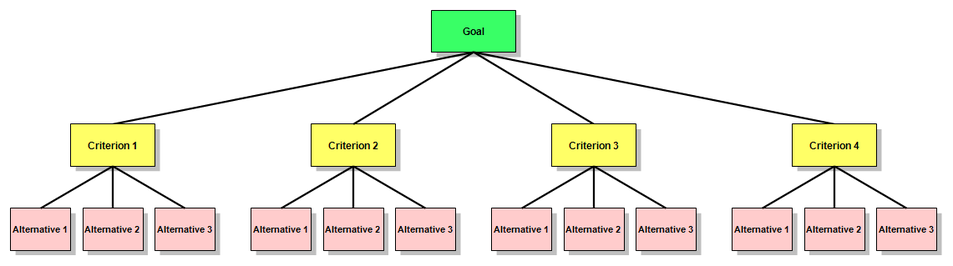
\includegraphics[width=1.05\textwidth]{AHP}
    \caption{AHP Hierarchy}
    \label{fig:AHP}
\end{figure}
\subsubsection{HOW IS AHP USED IN ALGORITHM ?}
Firstly, our algorithm takes the priority order of attributes and makes a comparison matrix M of size $n x n$. The value of element $M_i_j$ is (distance between Attribute $A_i$ and Attribute $A_j$ in the priority order + 1) if  and only if Attribute $A_i$ is prior to Attribute $Aj$. If Attribute $A_j$ is prior to Attribute $A_i$ then value of element $M_i_j$ is 1/\textit{(distance between Attribute $A_j$ and Attribute $A_j$ in the priority order + 1)}. After obtaining $M_i_j$, $M_j_i$ is calculated by inversing $M_i_j$.\\
For Example,

Algorithm takes the the priority order of  the user as $a , b , c , d $  which technically mean $ a > b > c > d $ then the corresponding comparison matrix of size $ 4 x 4 $ is as follows : 
\begin{table}[h!]
\centering
\caption{Comparison matrix.}
\vspace{0.1in}
 \begin{tabular}{|m{1cm}|m{1cm}|m{1cm}|m{1cm}|m{4em}|}
\hline
 & a & b & c& d\\
\hline
a& 1 & 2 & 3 & 4 \\
\hline
b & 1/2 & 1 & 2 & 3 \\
\hline
c & 1/3 & 1/2 & 1 & 2 \\
\hline
d & 1/4 & 1/3 & 1/2 & 1 \\
\hline
\end{tabular}
\end{table}
corresponding weights:\\
$Weight_a = 0.46$ , $weight_b = 0.27$ , $weight_c = 0.15$ , $weight_d = 0.09$
\subsection{SCORING ALGORITHMS}
\subsubsection{ALGORITHM-\textbf{1}}
This algorithm consists of following steps:\\\\
\textbf{Classification of Attributes:}\\
The main function of a match-making recommender system is to recommend profiles considering what user primarily wants, and thus increase user's overall satisfaction. To achieve this attributes are divided into two groups. This classification is based on the importance of attributes. The first group consist of attributes of high importance like religion, caste, occupation, diet, marital status, smoke and drinking habits. Other group consist of less important attributes like age, height, education, annual income, body type and complexion. Our algorithm makes sure that all the attributes belonging to the first group are perfectly matched while giving recommendations. And it then uses the less important attributes in scoring profiles. TABLE 2.2 shows each of these attributes along with its importance and some possible values that attribute would take. New possible values for any attribute can be added into implemented system.
\begin{table}[h!]
\centering
\caption{Attributes Importance and Possible Values.}
\vspace{0.1in}
\begin{tabular}{|m{1cm}|m{2cm}|m{2cm}|m{8.3em}|}
\hline
Sl. No. & Attribute & Importance & Possible values \\
\hline
1. & Age & Low & 20 to 35 \\
\hline
2. & Height & Low & 4.8 to 6.3 \\
\hline
3. & Religion & High & Hindu,Jain,Christian,
                      Parsi,Muslim,Sikh, 
                        Buddhist,Jewish \\
\hline
4. & Caste & High & Arya,Aggarwal,
                    Rajput,Sindhi,
                    Patel,Catholic,
                    Parsi,Buddhist,
                    Jewish,Pama,Teli,
                    Maratha,Brahmin,
                    Sunni,Shia,
                    Digamber,Vaishnav,
                    Protestant \\
\hline
5. & Education & Low & Doctors(PhD,Mphil),
                       Masters(ME,MTch,MSc,
                       MS,MD,MCm,MA),
                       Bachelors(BE,
                       BTech,BCom,BA,
                       BSc,BHMS,BAMS,
                       MBBS,BDS,LLB), 
                       Diploma(Diploma,
                       DMLT),HSC,Below
                       HSC(SSC,9th)
                        \\
\hline
6. & Occupation & High & Assistant,
                         Government,
                         Businessperson,
                         Consultant,
                         Designer,Doctor,
                         Lawyer,Principal,
                         Teacher,Professor,
                         Researcher,
                         Lecturer,
                         Lab technician  \\
\hline
7. & Annual Income & Low & 100,000Rs to 1,500,000 Rs  \\
\hline
8. & Body Type & Low& Slim, Athletic,
                      Average, Heavy \\
\hline
9. & Complexion & Low & Veryfair, Fair,
                        Wheatish, Dark \\
\hline
10. & Diet & High & Non-veg, Veg \\
\hline
11. & Smoke & High & Yes, No \\
\hline
12. & Drink & High & Yes, No \\
\hline
\end{tabular}
\end{table}
\newpage
The possible values of age, height and income attributes are distributed into ranges. In our system we considered eight possible ranges for each of these three attributes. One possible range allocation for age attribute is shown in TABLE 2.3.
\begin{table}[h!]
\centering
\caption{Possible Ranges and Representation of Age Attribute}
\vspace{0.1in}
 \begin{tabular}{|m{4cm}|m{8em}|}
 \hline
 Age & Representation\\
\hline
20-22 & 1 \\
\hline
22-24& 2  \\
\hline
24-26&3 \\
\hline
26-28 &4 \\
\hline
28-30 & 5 \\
\hline
30-32& 6\\
\hline
32-34& 7 \\
\hline
34- & 8 \\
\hline
\end{tabular}
\end{table}\\
For instance, a new female user has registered into the matrimonial site and she has specified partner preference attributes value as follows:
Age - 26 to 28, Height - 5.9 to 6, Religion - Hindu, Caste - Doesn't Matter, Education - BTech, Occupation - Engineer, Annual Income - 800,000 Rs. to 1,200,000 Rs., Body Type - Athletic, Complexion - Fair, Diet - Non-Veg, Smoke - No, Drink - No.
Then her preference attribute vector would be set as [5, 6, 1, 0, 4, 10, 4, 2, 3, 2, 1, 1]. Doesn't Matter is taken as 0.\\\\
\textbf{Shortlisting Users for N-Recommendations.}\\
This step produces an unordered list of recommendations for a user. The active user's preference attribute vector is compared against each of the profiles in opposite gender and a list of recommendations is generated where all the attributes of high importance matches perfectly. By doing this we avoid computing scores for all the users in the database, and also computational load on the system can be minimized as only few users will be considered for scoring discussed in the next step. This ensures that the n-recommendations given by our algorithm satisfies or suits the requirements of Indian marriage culture.\\\\
\textbf{Calculation of Similarity Index Between Two Users:}\\
The unordered list of N-recommendations generated in the previous step doesn't fulfill the complete purpose of a good recommender system (RS). In order to meet the personalized preferences of any user, a good RS must be able to display recommendations in some order unique for that user. This is discussed in this step.

As we have already used six high important attributes in the previous step of shortlisting recommendations, we will use the remaining six low important attributes in this step to achieve our purpose. Each of these six attributes contribute to the overall matching-score for a user-user comparison. 

For each of these six attributes, a similarity index is calculated between active user's preference value and other user's profile value for that attribute. This similarity index is multiplied by weight corresponding to that attribute.

For example, if we consider the attribute complexion, the four possible values for that attribute are $Very$ $Fair$, $Fair$, $Wheatish$ and $Dark$. Now if active user $A's$ complexion preference is $Wheatish$ and shortlisted users $B$, $C$, $D$, $E$ preferences for that attribute are $Dark$, $Wheatish$, $Fair$ and $Very$ $Fair$ respectively. Similarity index for each comparison is calculated by the formula:
	\[\textit{Similarity Index} = 1-dist * factor\]
Where $ dist$ is the distance between active user's preference value and other users profile value for that attribute

$factor$ is \[1/\textit{no of possible values for that attribute}\]\\
Now similarity indices for complexion\\

$A-C$ is 1- 0 = 1

$A-B$ and $A-D$ is 1-1 *0.25 = 0.75

$A-E$ is 1- 2*0.25 = 0.5\\\\
This method doesn't consider user's onsite behavior when calculating similarity-index, it just relies on user's preferences taken from him/her during signup. This can be accomplished by using user-user ratings data. For the same example discussed earlier, if user A has previously liked 100 users and among them 20 users falls under Dark complexion, 40 under Wheatish, 30: Fair and 10: Very Fair. Now the similarity index is calculated as\\

$A-C$ is \(\displaystyle \frac{40}{40} \) = 1\\

$A-B$ is \(\displaystyle \frac{20}{40} \) = 0.5\\

$A-D$ is \(\displaystyle \frac{30}{40} \)  = 0.75\\

$A-E$ is \(\displaystyle \frac{10}{40} \) = 0.25\\\\\\
This process is repeated for other five less important attributes to calculate corresponding similarity index.\\\\
\textbf{Aggregation Method and Ranking Users}\\
In this step, a final score is assigned to each user. For each less important attribute, similarity index is multiplied by attribute weight. Summation of all these multiplications gives the score for that particular user.\\
$$\textit{Score} = \sum_{i=1}^{6} similarity_i * weight_i$$
The shortlisted list is rearranged in descending order of their scores and ranks are assigned to them. Users are recommended to the active user in the order of these ranks.\\
 
\subsubsection{ALGORITHM-\textbf{2}}
Here we intake \textit{User Profile, User Preferential List, User Priority Order of Attributes and Order of Criteria.} User priority order of attributes and order of criteria are sent to AHP weighing algorithm to estimate the weights of the attributes. User Profile consists of information details of the user. User Preferential list consists of what attribute values are mostly preferred, lesser preferred and least preferred expecting from a opposite gender user. \\
Here, 10 Attributes are considered on the 3 different criterion :\\\\
\textbf{Education/Occupation}\\			                         (Educational Qualification,Occupation/Profession)\\\\
\textbf{Wealth}\\	                                                       (Earnings, Family Status, Location)\\\\
\textbf{Personality}\\                                                         (Age, Height, Complexion, Body type, Diet)\\\\
\textbf{\textit{Example :}}\\
\textbf{Attribute :} Diet	\\
\textbf{Existing Values :} Eggitarian, Vegetarian, Non Vegetarian\\\\
If a user prefers Vegetarian the most and ready to compromise if the user is  Eggitarian rather than Non Vegetarian. Then he fills the details as follows :\\
\textbf{Most Preferred:}
Diet : Vegetarian\\
\textbf{Preferred:} 
Diet : Eggitarian\\
\textbf{Least Preferred:}
Diet : Non Vegetarian\\\\
Upon assigning similarly for 10 other attributes into 3 categorial distribution of Preferences, we have a complete list of  User Preferential list.\\\\
\begin{figure}[h]
    \centering
    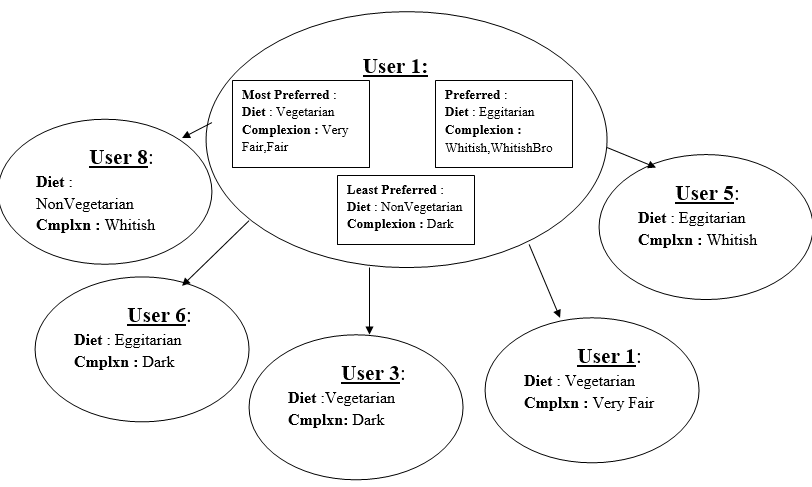
\includegraphics[width=1.05\textwidth]{upon}
    \caption{Mapping a Bridegroom Preferences with a Bride's Profile}
    \label{fig:upon}
\end{figure}
Let, W\textsubscript{complxn} be weight of complexion and  W\textsubscript{diet} be Weight of Diet\\
Assume,

W\textsubscript{complxn} = 0.35$, W\textsubscript{diet} = 0.01$\\\\
Score generated according to User1 preferential list :\\\\
\textbf{Level 1: (1, 100, 10000)}

$User 1 : 10000 * W\textsubscript{diet} + 10000 * W\textsubscript{complxn} = 3600$

$User 3 : 10000 * W\textsubscript{diet} +  1 * W\textsubscript{complxn} = 100.35$

$User 5 : 100 * W\textsubscript{diet}  + 100 * W\textsubscript{complxn} = 36$

$User 6 : 1* W\textsubscript{complxn} + 100 * W\textsubscript{diet} = 1.35$

$User 8 : 1* W\textsubscript{diet} + 100 * W\textsubscript{complxn} = 35.01$\\\\
Recommendation Order (Top 3) :

$Scoreuser1 > > > Scoreuser3 > Scoreuser5 == Scoreuser8 > Scoreuser6$\\\\
Here, algorithm works in such a manner that it tries only to show the users whose most preferred attribute value is matched i.e. by multiplying 10000 to the weightage of the attribute whose value gets matched.\\\\ 
\textbf{Level 2 : (1, 10, 100)}

$User 1 :  100 * W\textsubscript{diet} + 100 * W\textsubscript{complxn} = 36$

$User 3 : 100 * W\textsubscript{diet} +  1 * W\textsubscript{complxn} = 1.35$

$User 5 : 10 * W\textsubscript{diet}  + 10 * W\textsubscript{complxn} = 3.6$

$User 6 : 1* W\textsubscript{complxn} + 10 * W\textsubscript{diet} = 0.45$

$User 8 : 1* W\textsubscript{diet} + 10 * W\textsubscript{complxn} = 3.51$\\\\
Recommendation Order (Top 3) :

$Scoreuser1 > Scoreuser5 == Scoreuser8 > Scoreuser3 > Scoreuser6$\\\\
Algorithm tries to show the best matching user profiles from preferred category besides most preferred category.\\\\
\textbf{Level 3 : (1, 4, 16)} 

$User 1 :  16 * W\textsubscript{diet} + 16 * W\textsubscript{complxn} = 5.76$

$User 3 : 16 * W\textsubscript{diet} +  1 * W\textsubscript{complxn} = 0.51$

$User 5 : 4 * W\textsubscript{diet}  + 4 * W\textsubscript{complxn} = 1.44$

$User 6 : 1* W\textsubscript{complxn} + 4 * W\textsubscript{diet} = 0.39$

$User 8 : 1* W\textsubscript{diet} + 4 * W\textsubscript{complxn} = 1.41$\\\\
Recommendation Order (Top 3) :  

$Scoreuser1 > Scoreuser5 ===Scoreuser8 > Scoreuser3 == Scoreuser6$\\\\
Algorithm tries to show the matching user profiles from preferred category which user may like in addition to  most preferred category.\\\\
\textbf{Level 4 : (1, 2, 4)} 

$User 1 :  4 * W\textsubscript{diet} + 4 * W\textsubscript{complxn} = 1.44$

$User 3 : 4 * W\textsubscript{diet} +  1 * W\textsubscript{complxn} = 0.39$

$User 5 : 2 * W\textsubscript{diet}  + 2 * W\textsubscript{complxn} = 0.72$

$User 6 : 1* W\textsubscript{complxn} + 2 * W\textsubscript{diet} = 0.37$

$User 8 : 1* W\textsubscript{diet} + 2 * W\textsubscript{complxn} = 0.71$\\\\
Recommendation Order (Top 3) :

$Scoreuser1 > Scoreuser5 ==== Scoreuser8  > Scoreuser3 === Scoreuser6$\\\\
If user did not like any of the matches from prior levels then algorithm tries to show the best and better least preferred matches. \\\\
\subsection{COLLABORATIVE FILTERING BASED ALGORITHM}
\begin{figure}[h]
    \centering
    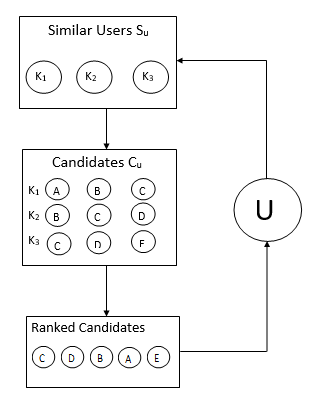
\includegraphics[width=0.9\textwidth]{cfa}
    \caption{Recommender Process}
    \label{fig:cfa}
\end{figure}\\
This collaborative approach calculates the similarities between same gender users relying on their preferences and then gives out recommendations from other gender that are expected to be successful in reciprocal order, based on the dislikes and likes of users in the similar list. By reciprocity we check if both the users being considered like each other or not. For example, if we consider a person $U$, we list out the users that $U$ is interested in, who also share interest in $U$. This means $U$ likes someone after seeing that person in his recommendations list and the response of this person was also positive.

The entire process of making recommendation in an ordered fashion comprises of three vital steps, see Figure 2.5. First, we find list the users $S_u$ belonging to same gender group as $U$ and are similar to $U$ by calculating the similarity co-efficient between the preference attributes. Then secondly, we examine the interactions of the users in $S_u$ with users from other gender and generate candidate recommendations $C_u$. Third, using reciprocity as the scoring parameter we assign ranks to users. These three steps are further discussed below.\\\\
\textbf{Generating Similar Users Based on User Preferences}\\
This is the first step in collaborative filtering approach, finding the similar users. If $U$ is the user under consideration, this step produces a list of K most similar users $S_u$ to $U$ in his/her own gender group. We take user $U's$ all twelve attribute preferences and find users with similar preferences. 

Distance metrics like Manhattan distance, Euclidean distance, cosine similarity, etc., can be employed for this purpose. More the distance between users, less the similarity between them. If the distance between two preferences vectors is 0, then that two persons are said to be identical. For our research, we have used Manhattan distance to calculate the distance. 
$$\textit{Distance(A,B)} = \sum_{i=1}^{12} PrefA_i - PrefB_i$$

Where $PrefA_i$ is $i$'th preference of user $A$\\\\
\textbf{Generating Candidates to be Considered for Recommendation Based on User Interaction}\\
The next step is to generate a list of candidate $C_u$. This list consists of all candidates to be considered for recommendation in an unordered fashion. Reciprocity is taken into account in deciding the users to be added into this list. For every user in similar users list ($S_u$), we draw out all the users that he/she shares a reciprocal interest with. This means for a user to join candidate list, he/she has to like any user in similar list and that user in $S_u$ should also like her back.  All the users who follow this criteria are included in Candidate list ($C_u$) and  become candidates for
recommendation. 

For example, in Figure 2.5 if $K1$, $K2$ and $K3$ are the similar users, $[A, B, C]$ is the set of users with reciprocal interest for $K1$ is, $[B, C, D]$ for $K2$: and for $K3$ it is $[C, D, E]$, then the union, $C$ $[A, B, C, D, E]$ gives the recommendation users list for that user.
To aggregate the first two steps, we start with a maximum distance threshold of 1. For a
given user $U$,  we calculate his preferences similarity co-efficient with all the users in same gender group and pick the $K$ most similar users into the similar list $S_u$. Then for each user in $S_u$, we add all the users he/she was reciprocally interested in to the candidate list. In the next step discussed below, each user in this candidate list is assigned a score based on his/her degree of reciprocity.\\\\
\textbf{Assigning Scores to Candidate Users}\\
The next step is to rank the users in candidate in the candidate list $C_u$ so that we can recommend to the user in that order. This can be achieved by assigning a level of support for all the users in candidate list by considering interactions between the users in similar list and the users in candidate list $C_u$. The criteria for any user's addition to candidate list is that they have to be reciprocally liked by at least one of the users in similar list. However, some candidates might have received positive interest from more than one $S_u$ user and responded to some positively and to others negatively. Thus, some candidates have more successful interactions with $S_u$ than others. Our ranking approach, uses this multiple reciprocity and calculates score for each user in candidate list and then candidates can be recommended to the user in descending order of their scores. 

For each candidate user $X$  in the candidate list, we calculate the number of times $X$
has a positive interaction with a user in similar list $S_u$. This included the events where he responded positively or received a positive response from a user in $S_u$, see Table 2.4. Now we calculate the count of negative interaction, number of times $X$ has responded negatively or has received a negative response from $S_u$. The number of positive minus the number of negative interactions of a user give his/her score in this system. The higher the score for user, the more he is reciprocally liked by users in $S_u$. The candidates are sorted in descending order based on their score and recommended to the user.
\begin{table}[h!]
\centering
\caption{Assigning of Scores to Candidate Users Based on Responses}
\vspace{0.1in}
 \begin{tabular}{|m{3cm}|m{4cm}|m{4cm}|m{2em}|}
 \hline
 Candidate & Positive responses & Negative responses & Score\\
\hline
A & 2 & 7 & -5\\
\hline
B & 6 & 5 & 1\\
\hline
C & 12 & 6 & 6\\
\hline
D & 6 & 2 & 4\\
\hline
\end{tabular}
\end{table}\\
Thus it can be ensured that users in candidate list who are reciprocally most liked by more  number of users in similar users list are always ranked ahead of candidates who are comparatively less liked. At the same time it also accounts for the over representation of popular candidates as they are more likely to have a higher negative response rate.
\newpage
\chapter{RESULTS AND DISCUSSIONS}
\section{RESULTS}
In the experimental setup, the proposed system is used to recommend exact or near exact matches who best satisfy the active user's requirements. Evaluation metrics like precision, recall and f-score can be used to evaluate the results of the recommender system.
\subsection{RESULTS FOR SCORING ALGORITHM - 1}
In this algorithm, two levels of calculation are done. Firstly, the entire database is searched to shortlist users who would satisfy the active user's high important attributes. Then his/her less important attributes are used along with his weights for those attributes to assign a score to each shortlisted user. Then these users are recommended in the order of their scores.

The preferences of a prospective bride is as follows:  age - 24 to 26, height - 5.9 to 6,    religion - Hindu, caste - Arya, education - Diploma,  occupation - Government, annual income - 8 lakhs  to 10 lakhs., body type - Average, complexion - Wheatish, Diet - Vegeterian, Smoke - No habits, Drink - No habits. The profiles in Table 3.1 are actives bride grooms in the system.
\begin{table}[h!]
\caption{Profiles of active bride grooms}
\vspace{0.1in}
 \begin{tabular}{|c|c|c|c|c|c|c|c|c|c|c|c|c|}
 \hline
 U-ID & Age & Hei & Rlgn & Caste & Edu & Occup & Incm & Body & Cmlx & Diet & Smo & Drnk\\
 \hline
 21 & 26 & 5.7 & Hindu & Arya  & Masters & Govt & 4L & Athl & Dark & Veg & No & No\\
 \hline
 22 & 24 & 5.5 & Hindu & Arya  & Doctors & Govt & 7L & Slim & Dark & Veg & No & No\\
 \hline
 23 & 30 & 5.1 & Hindu & Arya  & Doctors & Govt & 14L & Avg & Whtsh & Veg & No & No\\
 \hline
 24 & 22 & 4.10 & Hindu & Arya & HSC & Govt & 8L & Avg & Fair & Veg & No & No\\
 \hline
 25 & 26 & 5.2 & Hindu & Arya  & Bchlrs & Govt & 3L & Hvy & VFair & Veg & No & No\\
 \hline
\end{tabular}
\end{table}\\
If we run the algorithm on this data, the recommendations for active bride are shown in Table 3.2. For this sample data, we assumed that the weight of each attribute is 10.

\begin{table}[h!]
\centering
\caption{Recommendations for Active Bride}
\vspace{0.1in}
 \begin{tabular}{|m{3cm}|m{2em}|}
 \hline
 User-ID & Score\\
\hline
21 & 49.3\\
\hline
24 & 48.4\\
\hline
22& 46.45 \\
\hline
23 & 40.2 \\
\hline
25 & 44.65 \\
\hline
\end{tabular}
\end{table}

If the same user has already rated 140 profiles positively and out of those 140 users if 10 are in age-group(AG) 1, 10 in AG 2, 20 in AG 3, 30 in AG 4, 20 in AG 5, 10 in AG 6 and 20 each in AG 7 and 8. Similarly, if the distribution for $Height$ attribute is [10,10,10,30,30,10,10,30], for $Education$ attribute is [10,20,50,30,20,10], for $Annual$ $Income$ is [10,10,10,30,10,10,30,30], for $Body$ $Type$ is [20,20,40,60] and for $Complexion$ is [20,40,50,30], then the recommendations for the bride would be different as shown in Table 3.3. The system learns user's implicit preferences from his/her ratings and gives recommendations accordingly. 


\begin{table}[h!]
\centering
\caption{Advanced Recommendations for Active Bride}
\vspace{0.1in}
  \begin{tabular}{|m{3cm}|m{2em}|}
 \hline
 User-ID & Score\\
\hline
25 & 52.7\\
\hline
22 & 43.06 \\
\hline
21 & 41.73 \\
\hline
24 & 40.06 \\
\hline
23 & 38.06 \\
\hline
\end{tabular}
\end{table}
\subsection{RESULTS FOR SCORING ALGORITHM }
Upon applying the algorithm on the stated User-Bride data according to User-Bridegroom preferences,

Firstly algorithms results in the following order (Algorithm checks only Most Preferred (MP)):
\[3 > 4 > 6 > 5 > 7 > 2\]

If the user is not satisfied with the prior recommendations and ready to receive more recommendations (Algorithm checks the best among the leftover recommended Users (MP + Best (P))):
\[3 > 4 > 7 > 5 > 2 > 6\]

If the user is further does not get satisfied with the recommendations and ready to concede his Most Preferred preferences and want to check further more recommendations (MP + Better (P)  + Best(LP)):
\[3 > 4 > 7 > 2 > 5 > 6\]

If the user is ready to look over the whole database, then the algorithm is ready to display the recommendations according to the User’s perspective (MP + Almost(P) + Better(LP)) :
\[3 > 4 > 7 > 2 > 5 > 6\]\\
\begin{figure}[h]
    \centering
    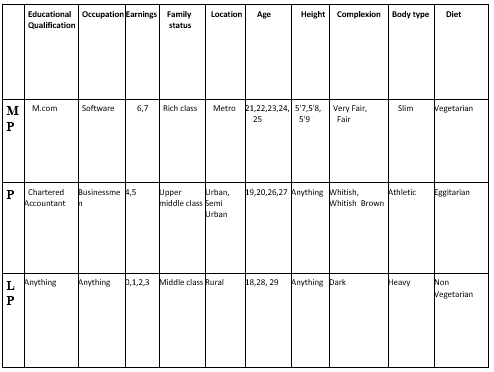
\includegraphics[width=1.0\textwidth]{table1}
    \caption{User-Bridegroom Preferential List}
    \label{fig:table1}
\end{figure}
\begin{figure}[h!]
    \centering
    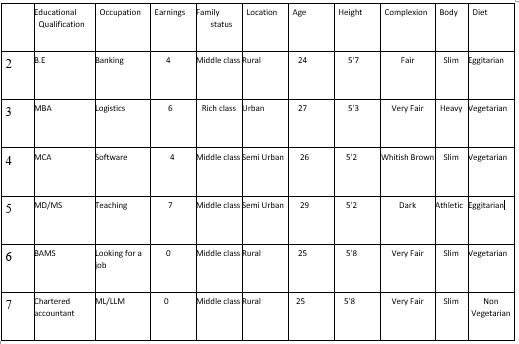
\includegraphics[width=1.2\textwidth]{table2}
    \caption{User-Bride Profile}
    \label{fig:table2}
\end{figure}

\newpage
\chapter{CONCLUSION AND FUTURE WORK}
\section{CONCLUSION}
Recommender systems have always been powerful as means of new technology that is used for proving to be an essence in  additional value for a business from its user databases. These systems help users find a commodity or an tradeable good that can be easily obtained from a business. Recommender systems benefit users by enabling them to find items they like. On contrary, these recommender systems help the business by generating more sales. Recommender systems are rapidly becoming a crucial tool in E-commerce on the Web. Recommender systems are being stressed by the huge volume of user data in existing corporate databases, and will be stressed even more by the increasing volume of user data available on the Web. New algorithms are of much need so as to dramatically improve the scalability of recommender systems.\\
This paper focuses on on explaining the vital importance of  improvisation over the existing recommender systems, which were much involved in getting more information from the user for knowing the partner preference that were much far away from providing perfect matches to their users. Our partially developed algorithm have shown that proposed recommender systems not only gives a new way of gaining information from users but also explains the mutual acceptance by providing matches with much similarity between them and not only are we providing N-recommendations but the order of each match that is provided to active user is taken into account, its an improvement in the field known less important.\\
\section{FUTURE WORK}
The following algorithm is partially developed and has the scope of improvement in the following areas:\\\\
1) The $Dataset$ - As this project requires a large dataset which is eventually obtained by big companies that is not readily available to use is the major drawback so we choose to test having a small sample of the data.\\\\
2) Like-factor is to be added. Level 5 recommendation is to be introduced where $\alpha$, $\beta$ are values strictly dependent on number of most preferred profiles, preferred profiles and finally least preferred profiles.\\\\
3) Weights of attributes can be changed based on user onsite behaviour.
\addcontentsline{toc}{chapter}{REFERENCES}
\bibliographystyle{unsrt}%Used BibTeX style is unsrt
\bibliography{ref}

\end{document}
